\section{Le client NextCloud}
%\addcontentsline{toc}{section}{Le client nextcloud}
Le nuage de \emph{apps} est basé sur le travail d'un groupe important de développeurs et de développeuses qui ont fondé le site et le serveur ``Nextcloud''. 
Ce service en ligne permet outre ce qui est offert par le nuage bien d'autres fonctionnalités. 

\begin{multicols}{2}

\begin{figure}
	\centering
	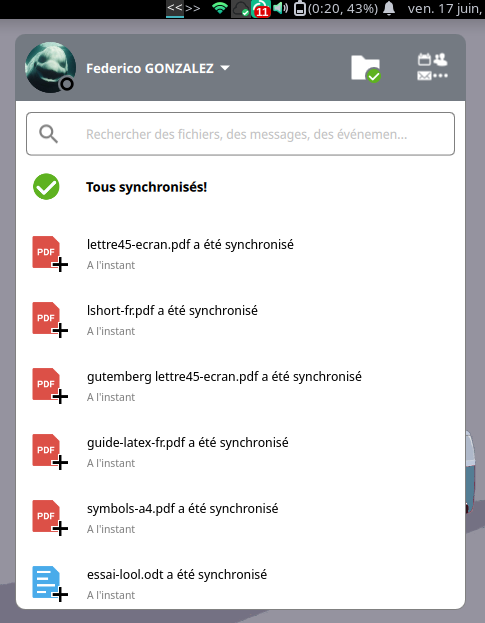
\includegraphics{./Captures/nextcloud-client.fenetre.principale.png}
	\caption{Le client pour PC (MacOS, Windows, ici : Linux}
\end{figure}

\columnbreak

\begin{figure}
	\centering
	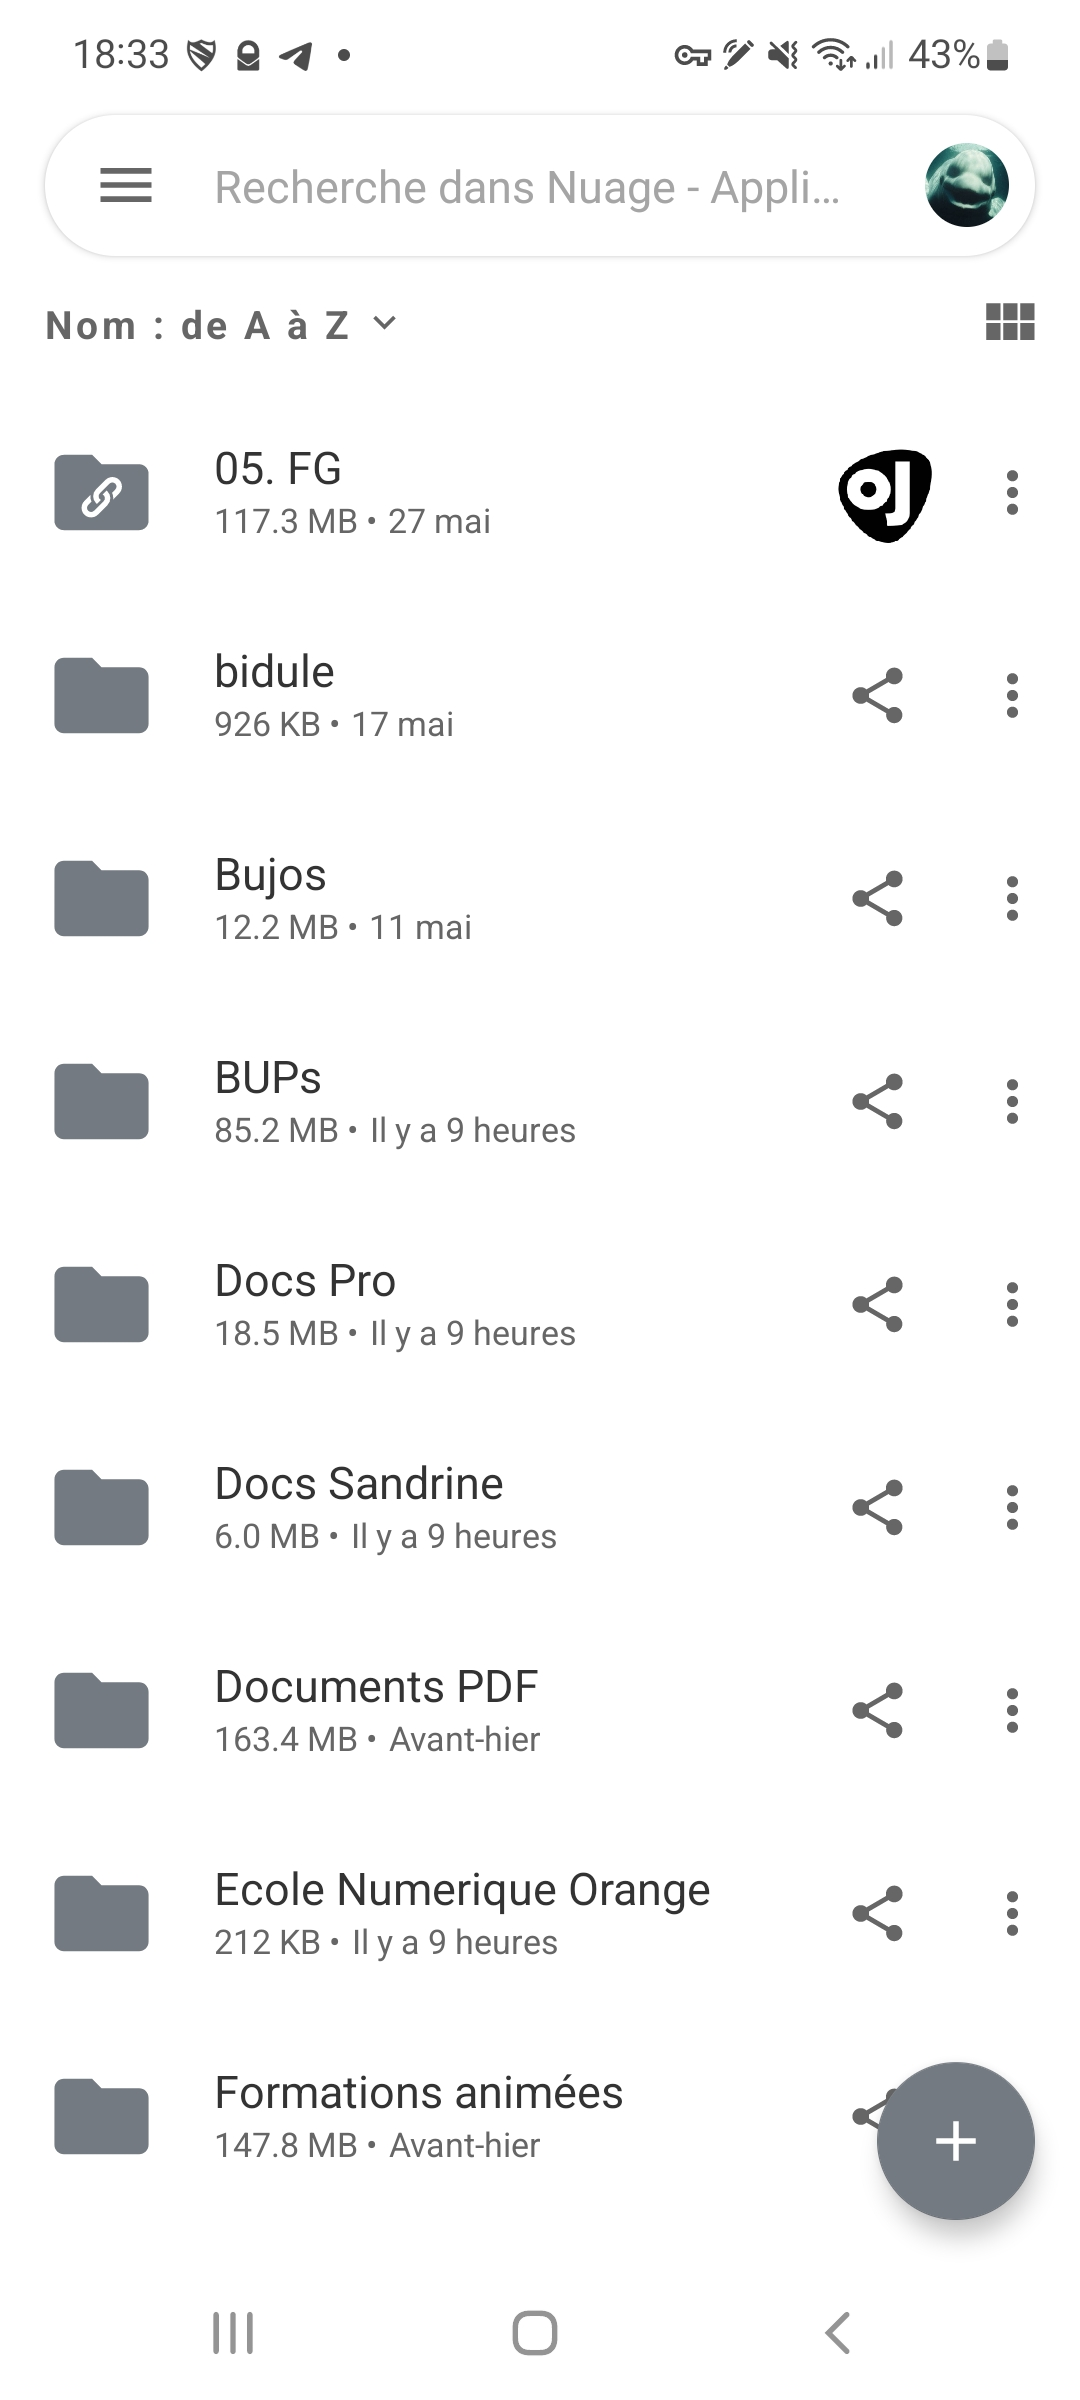
\includegraphics{./Captures/nextcloud-client.smartphone.jpg}
	\caption{Le client Nextcloud pour smartphone, version Android.}
\end{figure}
\end{multicols}
L'application est bien sûr disponible sur votre \emph{store\/}, quant au programme pour ordinateur il suffit d'aller sur le site \url{https://www.nextcloud.com} dans la section téléchargement.

Comment fonctionne le client Nextcloud pour PC~? 
C'est assez facile à comprendre. 
Lors de son installation, le client va demander un dossier, soit par défaut, soit en le spécifiant et en le créant, afin que tout fichier ou tout dossier qui y sera créé, supprimé, modifié, renommé, déplacé ou copié, sera synchronisé également sur le serveur automatiquement.
\begin{figure} \label{fig-dossier-synchro}
	\centering
	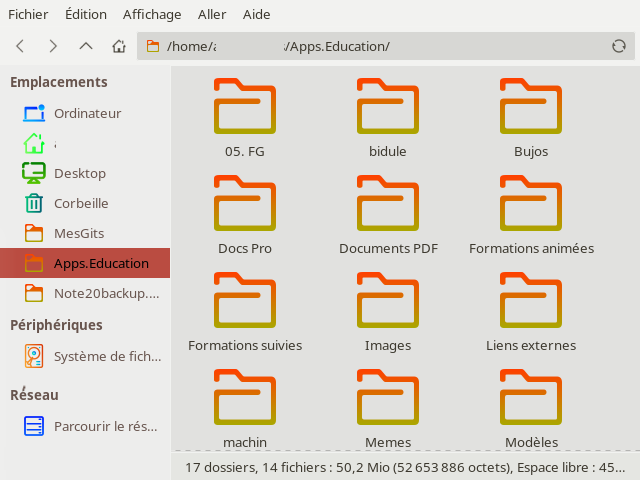
\includegraphics{./Captures/nextcloud-client.dossier.synchronise.png}
	\caption{Le dossier synchronisé sur mon P.C.}
\end{figure}

\paragraph{Notez.} 
Les prochaines sections et sous-sections traiteront de l'outil qui sera le plus souvent utilisé à savoir le transfert et la création d'objets par l'interface web, la gestion de tels échanges par le client nextcloud sera vu dans d'autres sections ultérieurement.